\documentclass[12pt, a4paper]{article}
\usepackage{graphicx}
\usepackage{url}

\title{Astronomy CNN with PyTorch}

\author{Axel Pontén}

\date{\today}

\begin{document}

\maketitle

Code is found at 

I implemented a CNN with two convolutional layers and two fully connected layers. I split 80/20 train/test. A few example spectra are shown in Fig. \ref{fig:spectra}.

\begin{figure}[!h]
    \centering
    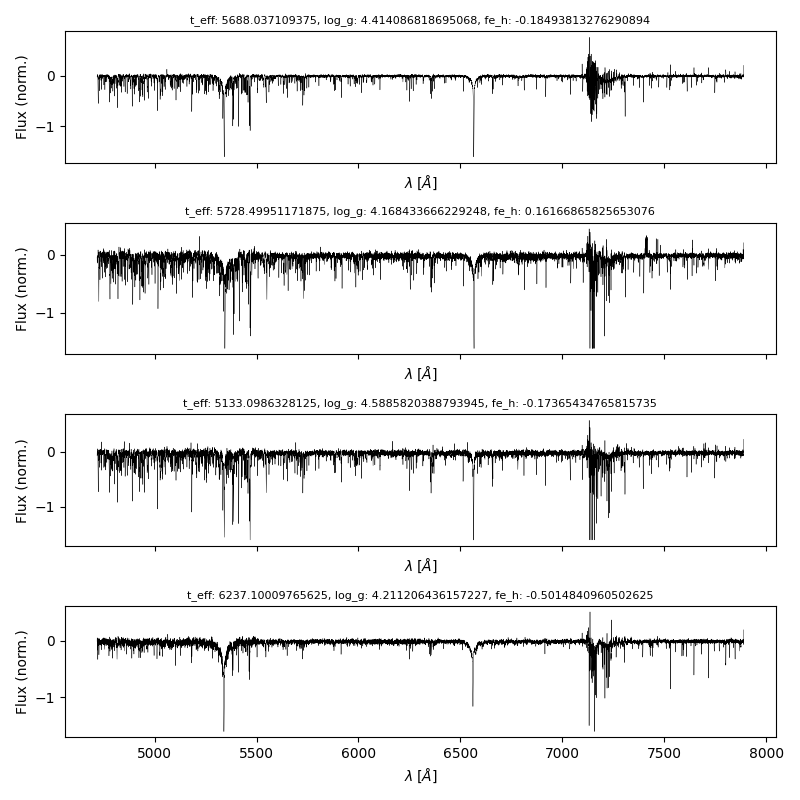
\includegraphics[width=0.6\textwidth]{../plots/spectra.png}
    \caption{Example spectra.}
    \label{fig:spectra}
\end{figure}


The input label distribution is shown in Fig. \ref{fig:label_dist}.
\begin{figure}[!h]
    \centering
    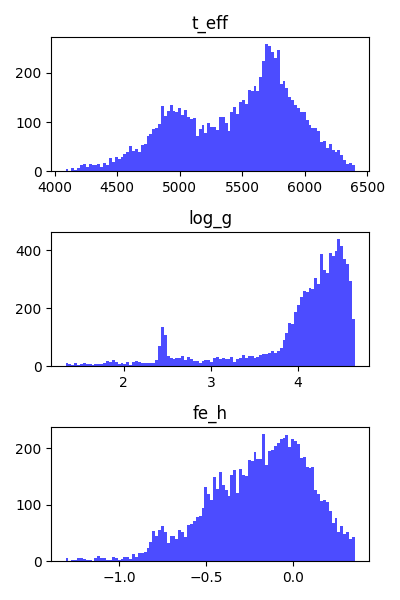
\includegraphics[width=0.4\textwidth]{../plots/normalize_target/labels.png}
    \caption{Label distribution.}
    \label{fig:label_dist}
\end{figure}

At first I didn't normalize target when training. I used MSE loss, but I have three labels which all have very different scale.
t\_eff is on the scale of ~5000 and fe\_h is on the scale of ~0.5.
Physically I'm interested in relative differences for the labels, but the network will react harder to 
differences in t\_eff than in fe\_h due to the absolute difference. For improvement I could
normalize the labels to have the same scale during training, and the reverse the transformation when using the network.

As you can see in Fig. \ref{fig:pred}, only t\_eff is predicted well. The other two labels are not predicted well.
After normalizing the labels to the label mean and std before training I get much better prediction as seen in Fig. \ref{fig:pred_norm}.

\begin{figure}[!h]
    \centering
    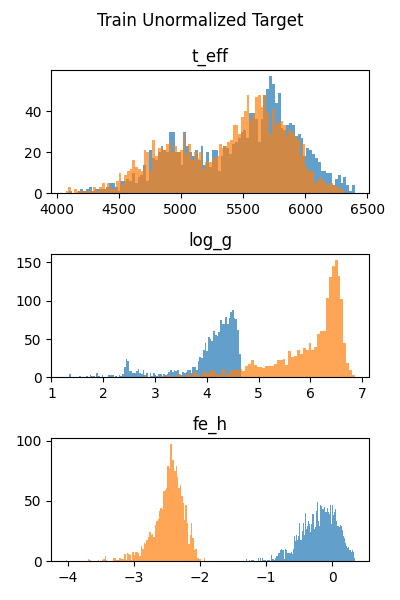
\includegraphics[width=0.4\textwidth]{../plots/pred.png}
    \caption{Prediction without normalizing labels.}
    \label{fig:pred}
\end{figure}

\begin{figure}[!h]
    \centering
    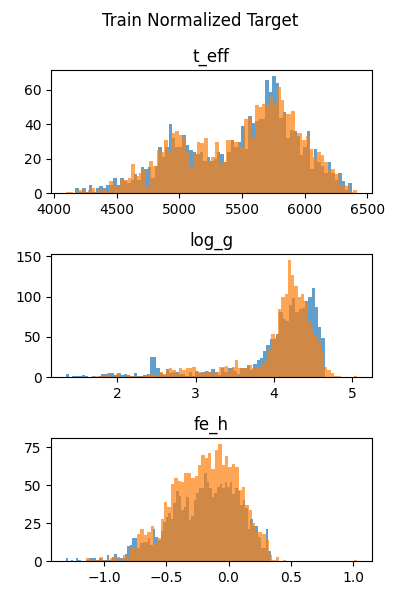
\includegraphics[width=0.4\textwidth]{../plots/normalize\_target/pred.png}
    \caption{Prediction after normalizing labels and training.}
    \label{fig:pred_norm}
\end{figure}

\end{document}